\subsection{Metoder (10 poeng)}\label{metoder-10-poeng}

% \begin{itemize}
% \item
%   Beskriv metodene dere bruker i prosjektet, og forklar i detalj hvordan
%   dere har anvendt dem. Dere bør bruke metoder fra mist 2 av de 3
%   temaene i kurset (regresjon, klassifikasjon, klyngeanalyse).
% \item
%   Forklar kort hvorfor metodene passer for datasett og problemstillingen
%   dere har valgt.
% \item
%   \textbf{Det er viktig at dere bare bruker metoder som er tilpasset
%   nivået i dette kurset -- bruk bare metoder dere lærer om her. Hold det
%   enkelt og realistisk, ikke bruk komplekse metoder som dere ikke
%   forstår, bare fordi KI foreslår det.}
% \item
%   Beskriv hvordan dere evaluerer metodene, hvis det er mulig. Evaluer
%   modellen(e) ved å bruke passende verktøy, for eksempel residualanalyse
%   eller vurdering av prediksjonsytelse (som sensitivitet og spesifisitet
%   i en binær klassifiseringsoppgave).
% \item
%   (Valgfritt) Diskuter mulige begrensninger ved metodene og de valgte
%   evalueringsmålene. Vurder for eksempel om et bestemt mål kan gi et
%   misvisende bilde av modellens ytelse, eller om det finnes egenskaper
%   ved datasettet som gjør en metode mindre egnede.
% \end{itemize}

I dette prosjektet kombinerer vi metoder fra to av hovedtemaene i kurset: \textbf{uovervåket klyngeanalyse} ($k$-Means, hierarkisk klyngeanalyse og PCA) og \textbf{veiledet klassifikasjon} ($K$-nærmeste naboer og logistisk regresjon). Denne kombinasjonen passer svært godt til problemstillingen vår: Først undersøker vi hvilke naturlige grupperinger som oppstår i de syv standardiserte lydvariablene ($Z$-verdier fra kapittel 3) uten at modellen kjenner til sjangrene, og deretter tester vi hvor mye bedre vi kan predikere de fem sjangerfamiliene når en klassifikasjonsmodell faktisk får lære sammenhengen mellom lydegenskaper og sjanger fra treningsdata.

\subsubsection{Tema 1: Uovervåket klyngeanalyse ($k$-Means, hierarkisk klyngeanalyse og PCA)}
For å finne naturlige grupperinger i lyddataene benytter vi \textbf{$k$-Means klyngeanalyse}. $k$-Means deler de $n = 2500$ sangene inn i $k$ disjunkte klynger $C_1, \dots, C_k$ ved å minimere den totale kvadrerte euklidske avstanden (Within-Cluster Sum of Squares, WCSS / Inertia) fra hver sang $z_i$ til klyngesenteret $\mu_c$ i klyngen den tilhører:
\[
\text{WCSS} = \sum_{c=1}^{k} \sum_{z_i \in C_c} \| z_i - \mu_c \|^2
\]
Algoritmen initialiserer $k$ klyngesentre og veksler iterativt mellom (1) å tilordne hver sang til det nærmeste klyngesenteret målt i euklidsk avstand, og (2) å oppdatere hvert klyngesenter som gjennomsnittsvektoren av sangene i klyngen, helt til konvergens.

For å velge antall klynger $k$ evaluerte vi $k \in \{2, \dots, 10\}$ ved hjelp av albue-metoden (WCSS) og gjennomsnittlig silhuett-score (figur~\ref{fig:elbow_silhouette}). Vi valgte $k = 5$ klynger, både fordi fallet i WCSS avtar merkbart rundt $k = 4\text{--}5$, og fordi $k = 5$ gir en direkte én-til-én-sammenligning med de fem overordnede sjangerfamiliene i datasettet.

\begin{figure}[htbp]
    \centering
    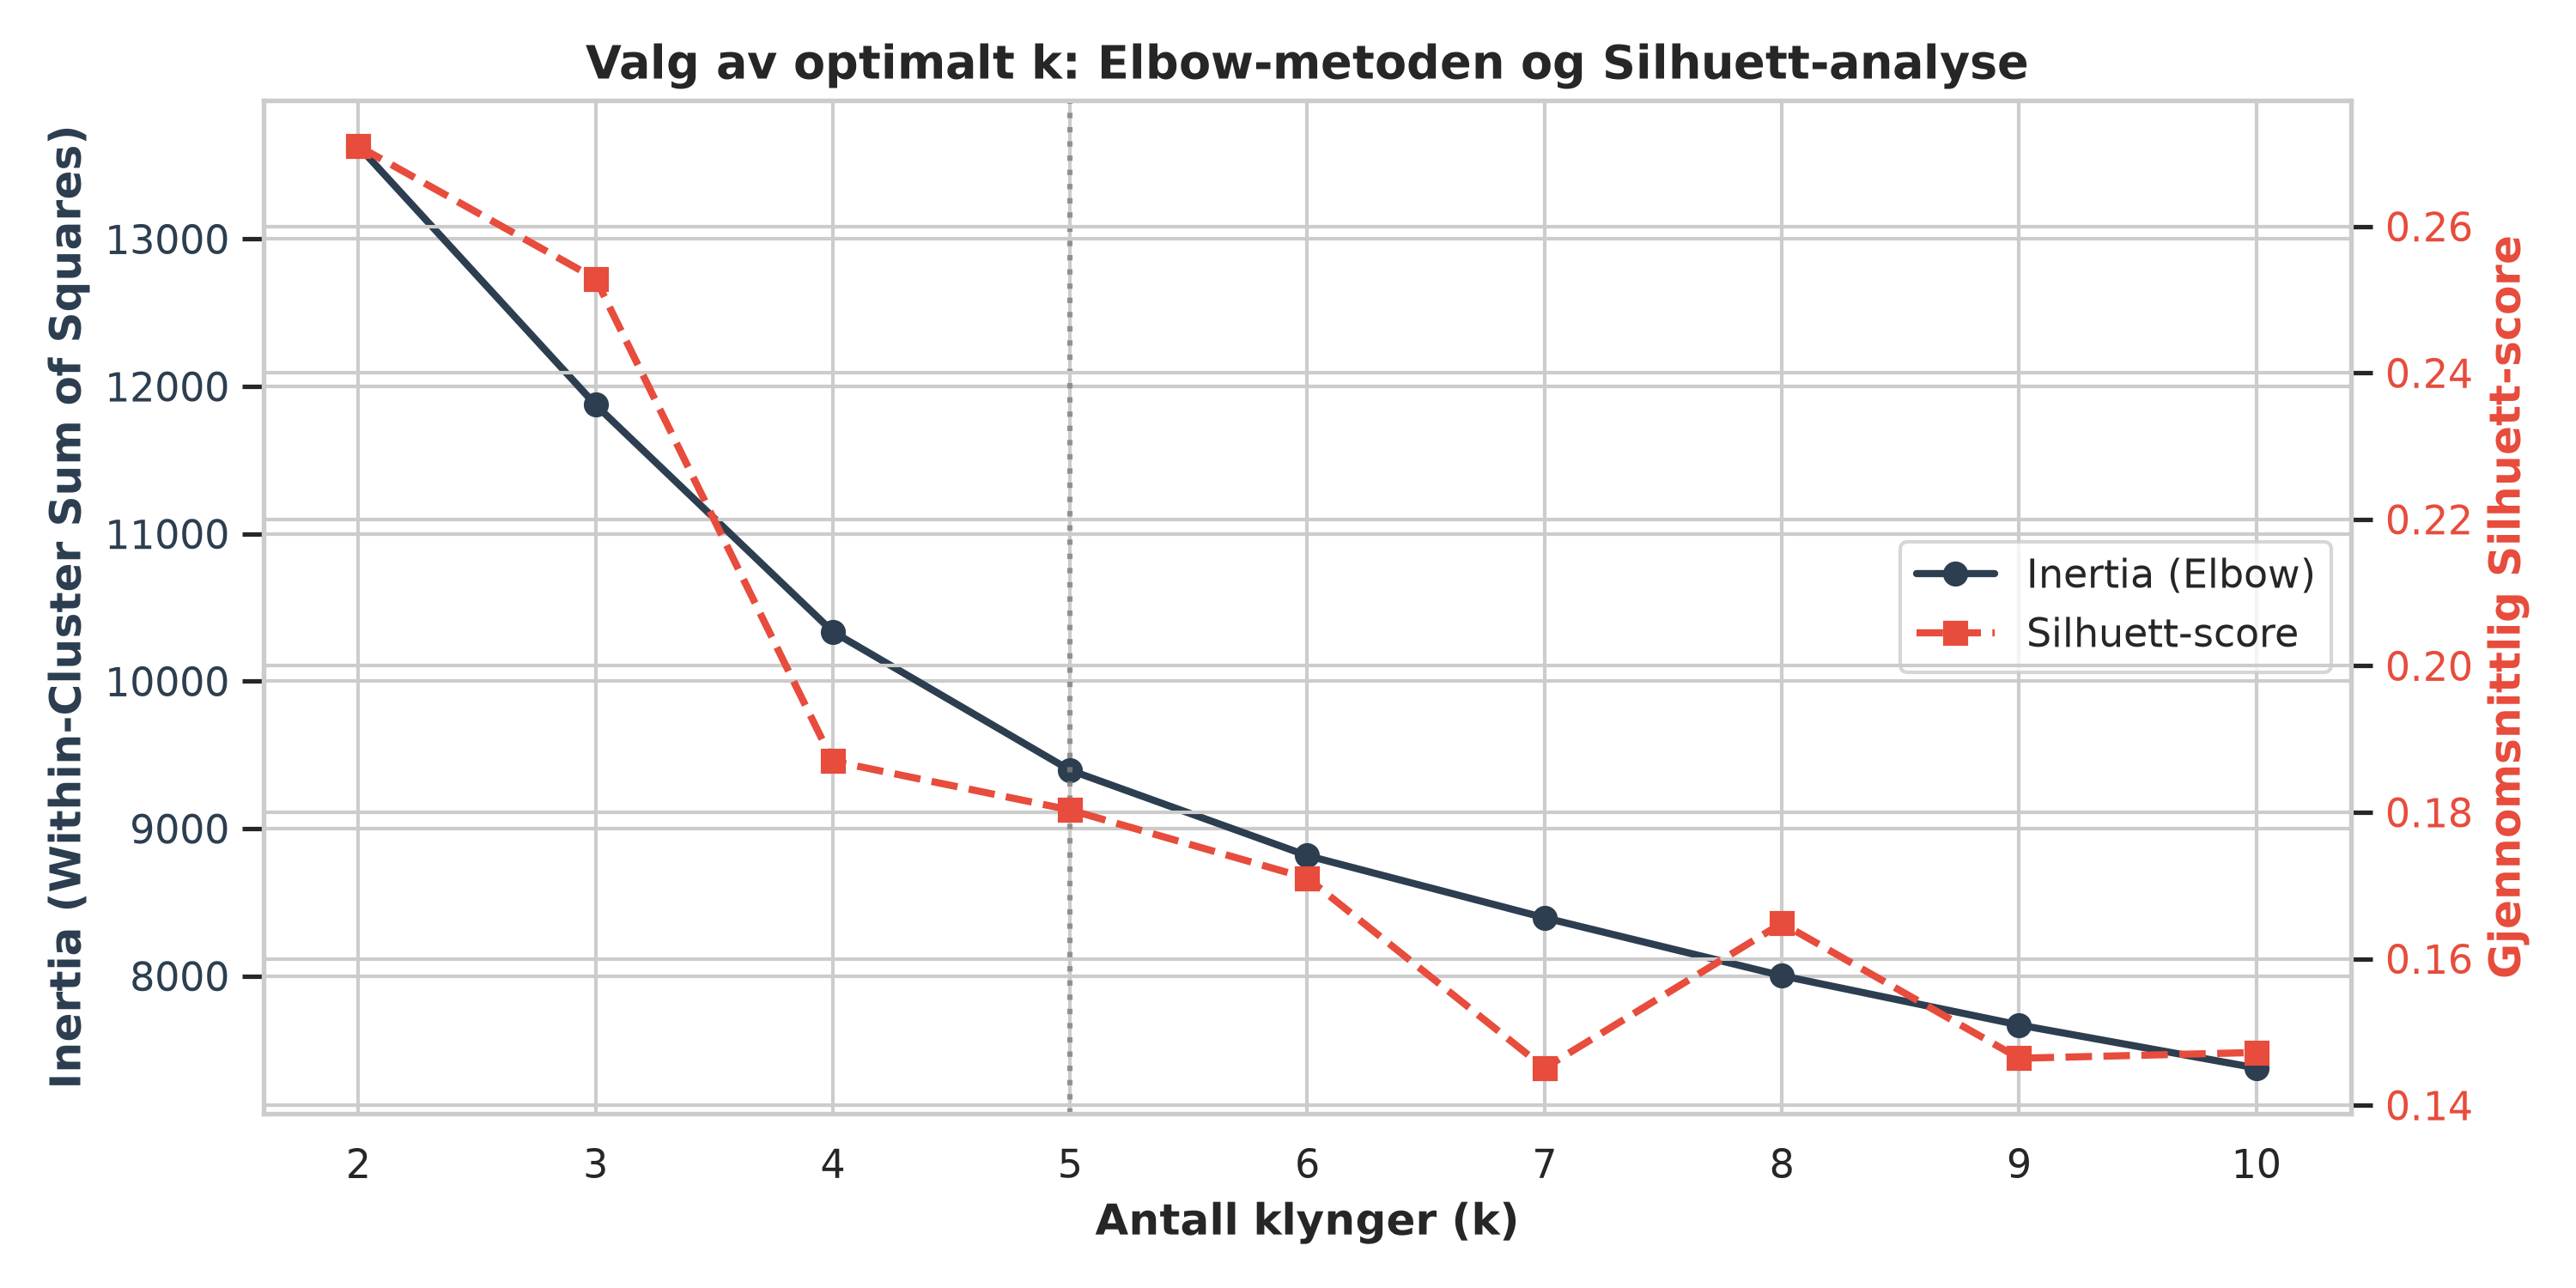
\includegraphics[width=0.88\linewidth]{figurer/1_elbow_and_silhouette.png}
    \caption{Valg av antall klynger $k$ for $k$-Means: WCSS / Inertia (albue-metoden, venstre akse) og gjennomsnittlig silhuett-score (høyre akse) for $k \in \{2, \dots, 10\}$. Den stiplede linjen markerer valgt $k = 5$.}
    \label{fig:elbow_silhouette}
\end{figure}

Som et supplement gjennomførte vi \textbf{agglomerativ hierarkisk klyngeanalyse} med \textbf{Wards kobling} på et tilfeldig utvalg på 100 sanger (figur~\ref{fig:dendrogram}). Algoritmen starter med hver sang som sin egen klynge nederst i et tre (dendrogram), og slår trinnvis sammen de to klyngene som gir minst økning i total innenfor-klynge-varians. Ved å kutte dendrogrammet horisontalt ved avstand $d = 10{,}5$ får vi fem hovedgrener, som lar oss kontrollere om en hierarkisk metode uten forhåndsbestemt $k$ støtter klyngestrukturen fra $k$-Means.

\begin{figure}[htbp]
    \centering
    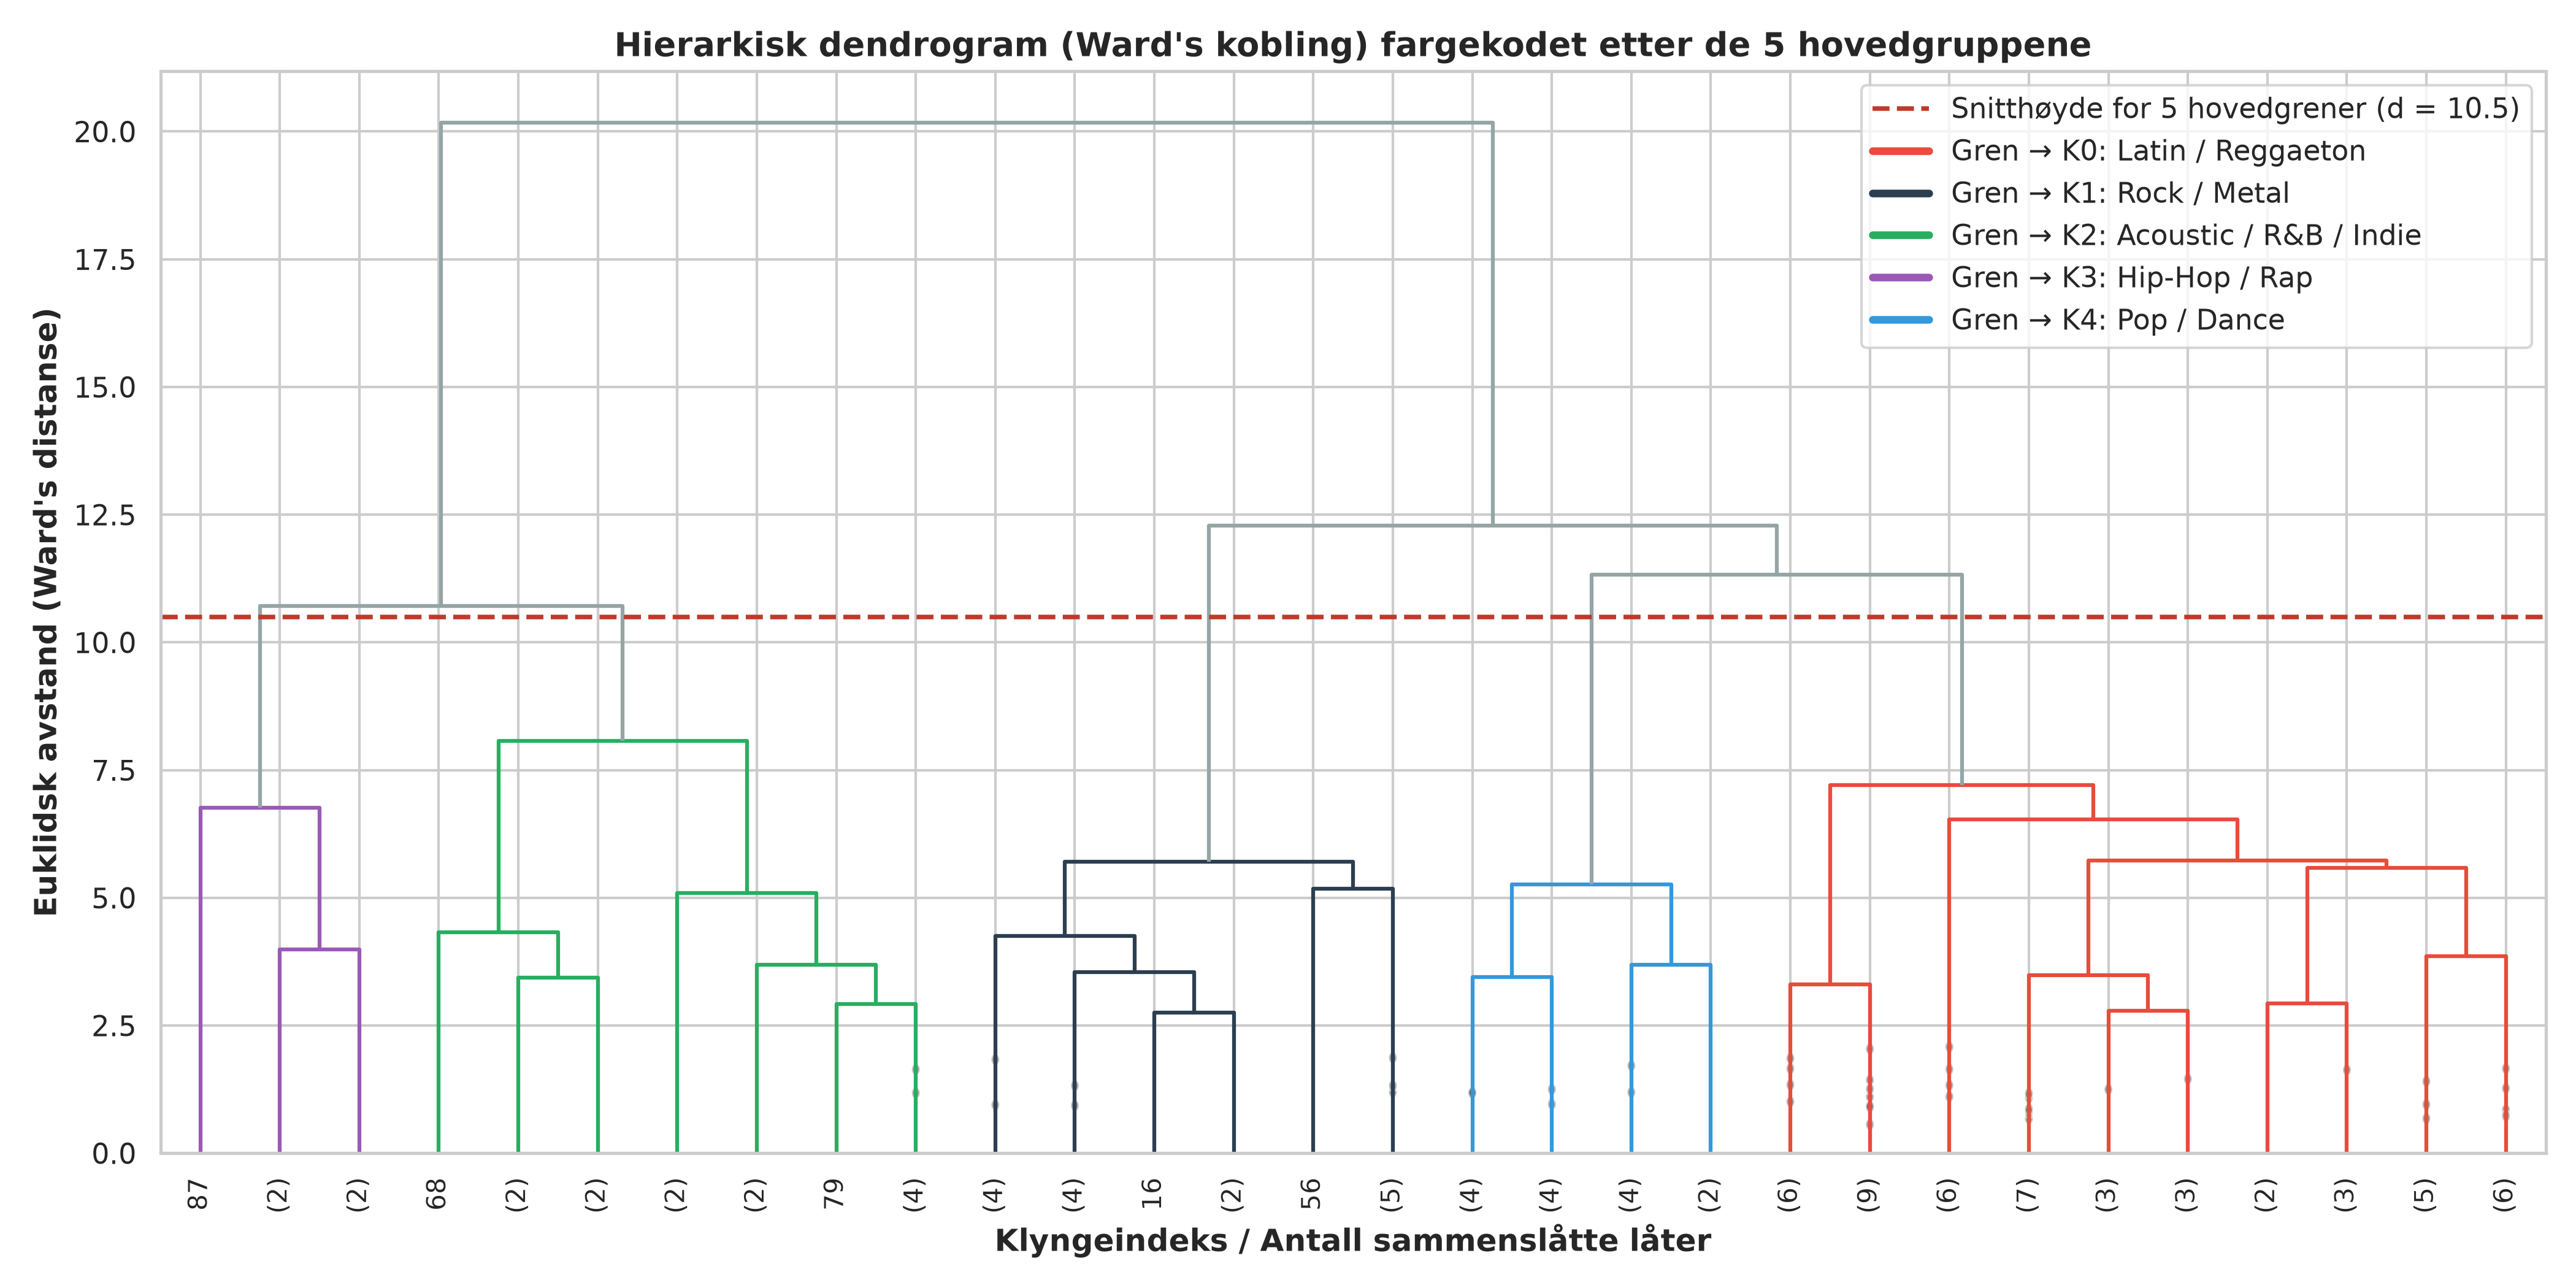
\includegraphics[width=0.95\linewidth]{figurer/4_hierarchical_dendrogram.png}
    \caption{Hierarkisk dendrogram med Wards kobling for et tilfeldig utvalg på 100 sanger. Den røde stiplede linjen ved avstand $d = 10{,}5$ markerer snitthøyden for 5 hovedgrener, fargekodet etter tilhørende $k$-Means-klynge.}
    \label{fig:dendrogram}
\end{figure}

Fordi klyngene befinner seg i et syvdimensjonalt rom, bruker vi \textbf{hovedkomponentanalyse (PCA)} for å visualisere klyngene i to dimensjoner. PCA konstruerer ortogonale lineærkombinasjoner av de syv variablene ($\text{PC1}$ og $\text{PC2}$, som til sammen forklarer $52{,}3\,\%$ av den totale variansen), slik at vi kan plotte både klynger og faktiske sjangre i samme todimensjonale koordinatsystem.

\subsubsection{Tema 2: Veiledet klassifikasjon ($K$-nærmeste naboer og logistisk regresjon)}
I prosjektets andre del formulerer vi sjangeridentifikasjon som en \textbf{veiledet klassifikasjonsoppgave} på de $n = 1566$ sangene som har kjent sjanger i datasettet. Her er de syv lydvariablene prediktorer $\mathbf{x}_i$, mens sjangerfamilien (\texttt{Genre\_Family} med 5 klasser) er den kategoriske responsvariabelen $y_i$. Vi deler disse sangene stratifisert inn i et \textbf{treningssett på $80\,\%$} ($1252$ sanger) og et uavhengig \textbf{testsett på $20\,\%$} ($314$ sanger), slik at sjangrenes relative fordeling er lik i begge sett. Standardiseringen ($Z$-score) tilpasses kun på treningssettet og brukes deretter til å transformere testsettet for å unngå datalekkasje.

Vi anvender og sammenligner to klassifikasjonsmetoder fra pensum:
\begin{enumerate}
\tightlist
\item
  \textbf{$K$-nærmeste naboer (KNN):} En ikke-parametrisk metode som klassifiserer en ny sang i testsettet ved å finne de $K$ sangene i treningssettet som ligger nærmest i euklidsk avstand i det syvdimensjonale lydrommet, og tilordne sangen til den sjangeren som har flertall blant disse $K$ naboene:
  \[
  \hat{P}(Y = j \mid X = \mathbf{x}_0) = \frac{1}{K} \sum_{i \in \mathcal{N}_0} I(y_i = j)
  \]
  Valget av hyperparameteren $K$ styrer avveiningen mellom skjevhet og varians (bias--variance tradeoff): lav $K$ gir en fleksibel grense med høy varians (fare for overtilpasning), mens høy $K$ gir jevnere beslutningsgrenser. Ved hjelp av 5-fold kryssvalidering på treningssettet for odde verdier $K \in \{1, 3, \dots, 35\}$ fant vi at $K = 15$ ga høyest kryssvalidert treffsikkerhet ($53{,}5\,\%$, figur~\ref{fig:knn_k}).
\item
  \textbf{Multinomial logistisk regresjon:} En parametrisk lineær klassifikasjonsmodell som estimerer sannsynligheten for hver av de $M = 5$ sjangerklassene ved hjelp av en lineær prediktor $\eta_{ik} = \beta_{0k} + \boldsymbol{\beta}_k^\top \mathbf{z}_i$ og softmax-funksjonen:
  \[
  P(Y_i = k \mid \mathbf{z}_i) = \frac{e^{\beta_{0k} + \boldsymbol{\beta}_k^\top \mathbf{z}_i}}{\sum_{m=1}^{M} e^{\beta_{0m} + \boldsymbol{\beta}_m^\top \mathbf{z}_i}}
  \]
  Ved å sammenligne logistisk regresjon (lineære klassegrenser) med KNN (ikke-lineære, lokale klassegrenser) får vi undersøkt om sjangergrensene i lydrommet er lineære eller mer sammensatte.
\end{enumerate}

\begin{figure}[htbp]
    \centering
    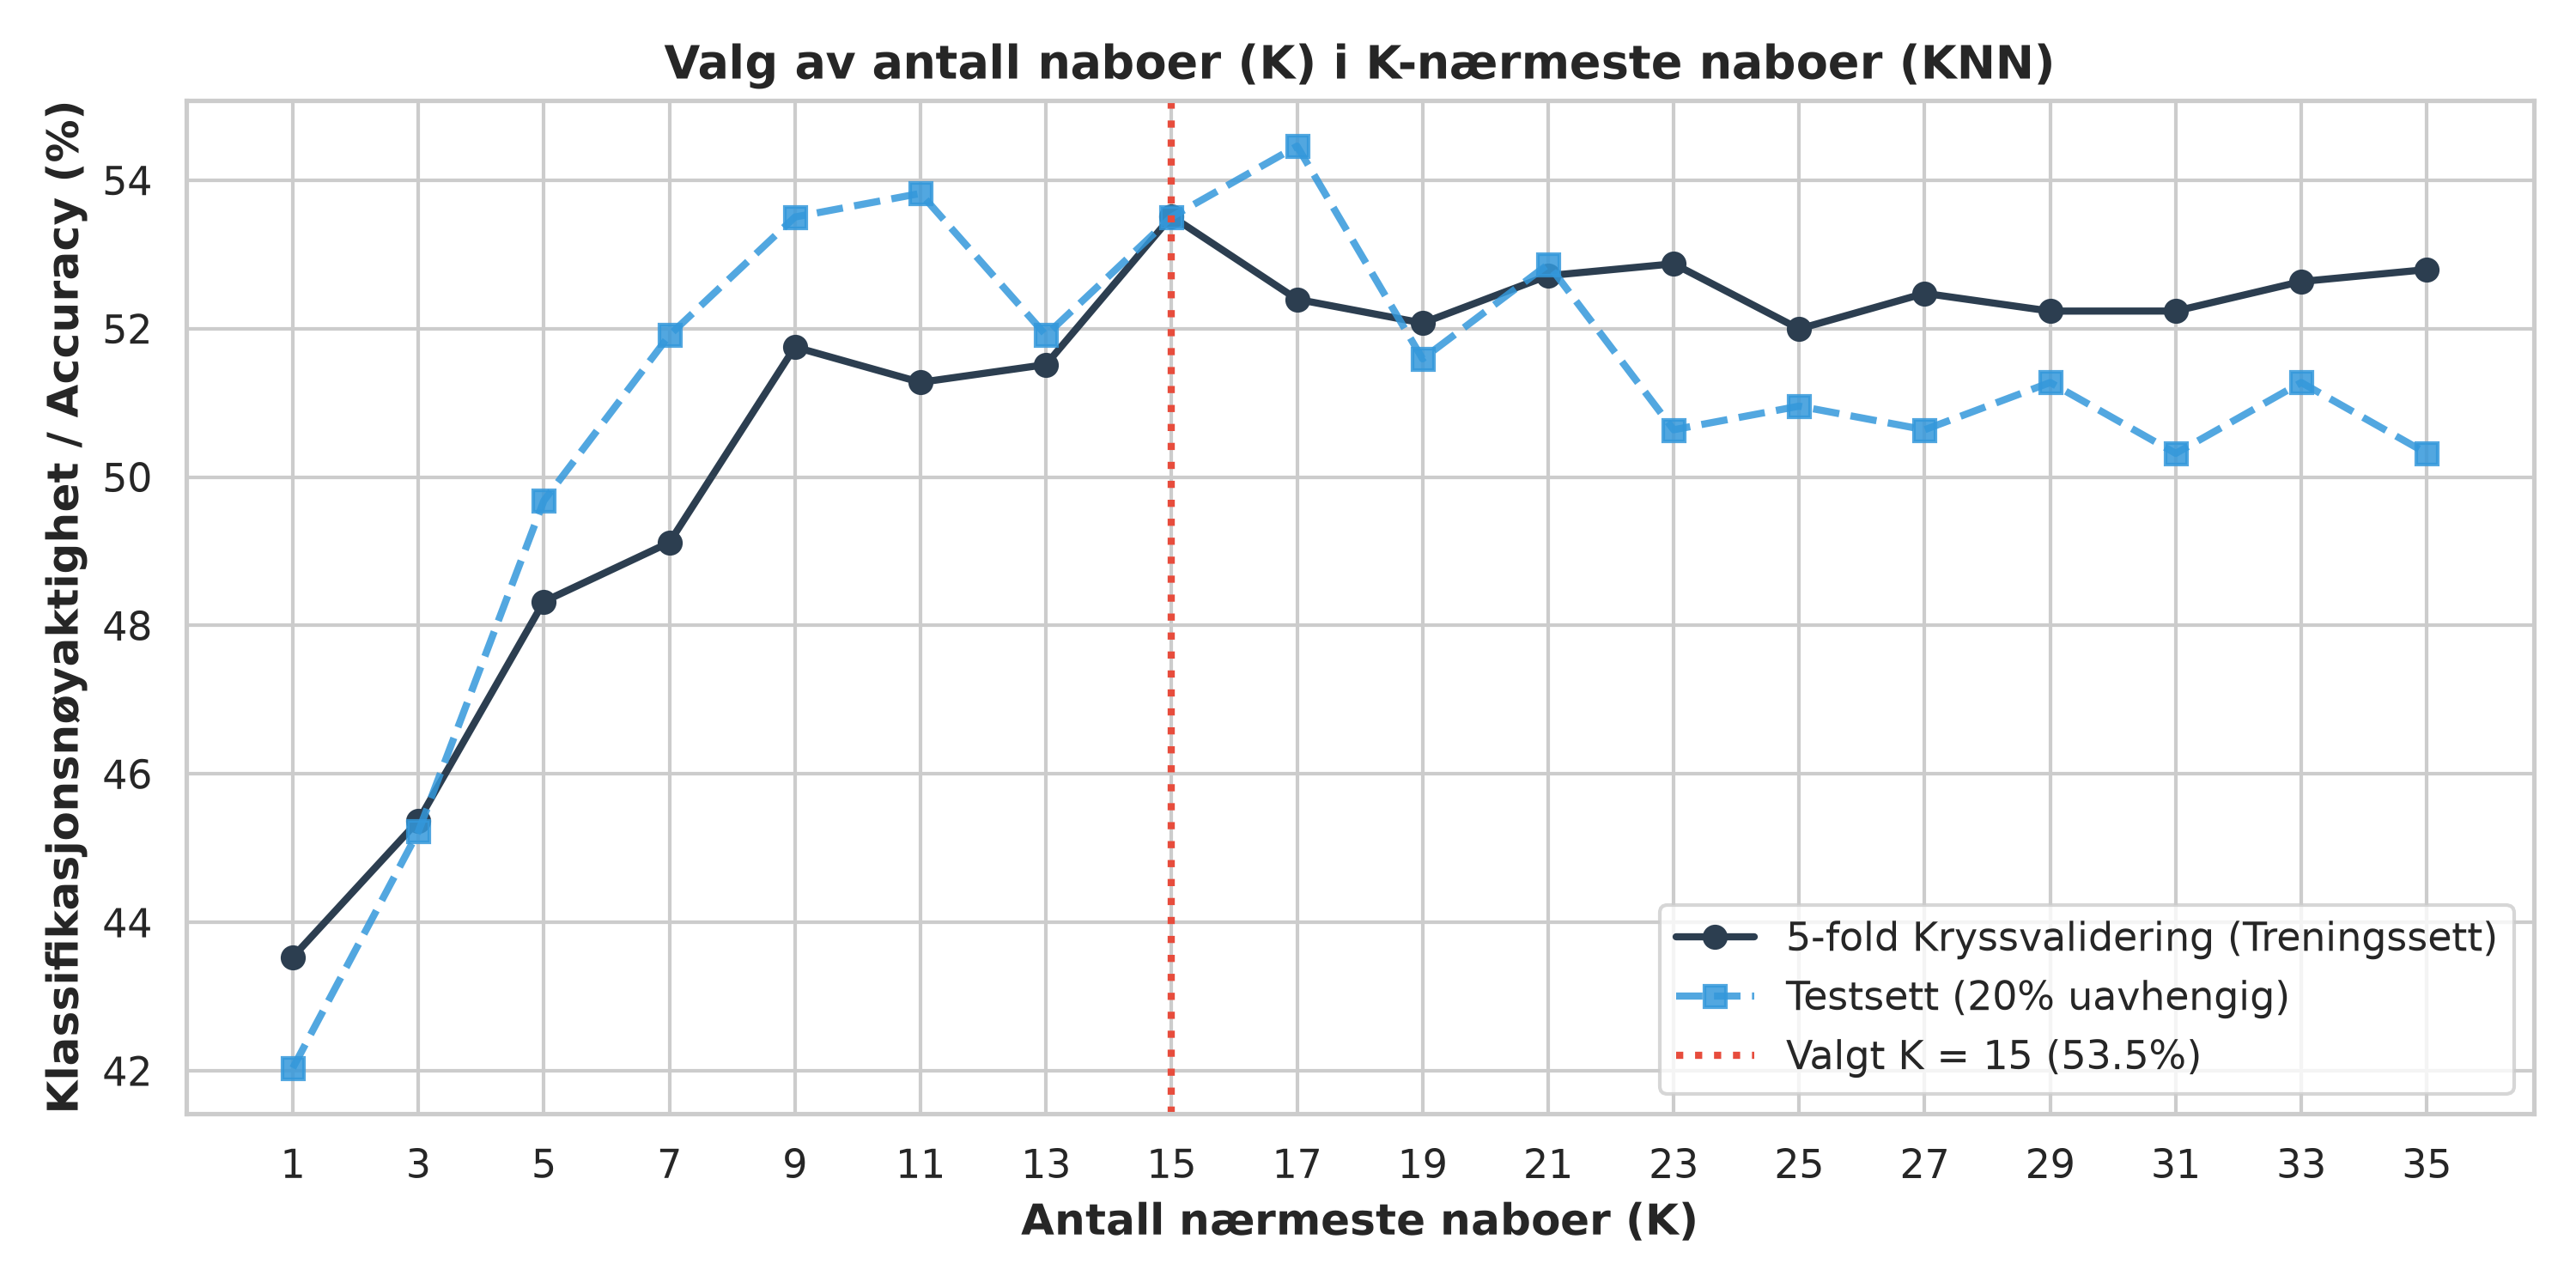
\includegraphics[width=0.88\linewidth]{figurer/7_knn_k_selection.png}
    \caption{Valg av antall naboer $K$ i KNN via 5-fold kryssvalidering på treningssettet ($n = 1252$) sammenlignet med nøyaktighet på testsettet ($n = 314$). Maksimal kryssvalidert nøyaktighet oppnås ved $K = 15$ ($53{,}5\,\%$).}
    \label{fig:knn_k}
\end{figure}

\subsubsection{Evaluering og metodiske begrensninger}
Vi evaluerer metodene med verktøy tilpasset henholdsvis uovervåket og veiledet læring:
\begin{itemize}
\tightlist
\item
  \textbf{Evaluering av klyngeanalyse:} Internt vurderes klyngene med WCSS, silhuett-koeffisienten $s(i) = \frac{b(i) - a(i)}{\max(a(i), b(i))}$ og klyngesentrenes $Z$-score-profiler. Eksternt vurderes klyngene i en kvadratisk ($5 \times 5$) krysstabell mot de fem sjangerfamiliene.
\item
  \textbf{Evaluering av klassifikasjon:} Klassifikasjonsmodellene evalueres på det uavhengige testsettet ($n = 314$) ved hjelp av total treffsikkerhet (\textit{Accuracy}, andel korrekt klassifiserte sanger), en kvadratisk ($5 \times 5$) \textbf{forvirringsmatrise} (\textit{confusion matrix}), samt klassevis \textbf{sensitivitet / recall} ($\frac{\text{TP}}{\text{TP} + \text{FN}}$, hvor stor andel av sangene i en faktisk sjanger modellen fanger opp) og \textbf{presisjon} ($\frac{\text{TP}}{\text{TP} + \text{FP}}$, hvor ofte modellen har rett når den predikerer en gitt sjanger).
\end{itemize}

Det er viktige begrensninger ved både metodene og evalueringsmålene. For det første antar $k$-Means sfæriske klynger av lik utstrekning, mens logistisk regresjon kun kan trekke lineære beslutningsgrenser mellom sjangrene. For det andre er klasseinndelingen i datasettet noe ubalansert (\textit{Pop / Dance} utgjør $434$ sanger, mens \textit{Acoustic / R\&B / Indie} kun utgjør $162$ sanger). I ubalanserte datasett kan total \textit{Accuracy} alene gi et skjevt bilde fordi en modell som favoriserer den største klassen (\textit{Pop / Dance}) oppnår høy total treffsikkerhet på bekostning av lav sensitivitet for mindre klasser. Nettopp derfor supplerer vi \textit{Accuracy} med klassevis sensitivitet (recall), presisjon og hele $5 \times 5$-forvirringsmatrisen. Endelig innebærer generaliseringen av 307 Spotify-undersjangre til fem hovedfamilier at sanger med overlappende stil eller hybride trekk (f.eks.\ pop-rap eller rolige pop-ballader) har en uklar fasit, noe som setter et naturlig tak for hvor høy treffsikkerhet enhver modell basert kun på syv lydmål kan oppnå.
